\subsection{Spyskaart en bestelling onderdeel}

Die spyskaart en bestelling onderdeel is die kernfunksionaliteit van die
stelsel wat gebruikers toelaat om spyskaarte te besigtig, bestellings te
plaas, en administrateurs toelaat om spyskaarte en bestellings te bestuur.
Dit sluit ook die gedetailleerde besigtiging van maaltye en die hantering
van bestelling geskiedenis in.

\begin{figure}[H]
    \centering
    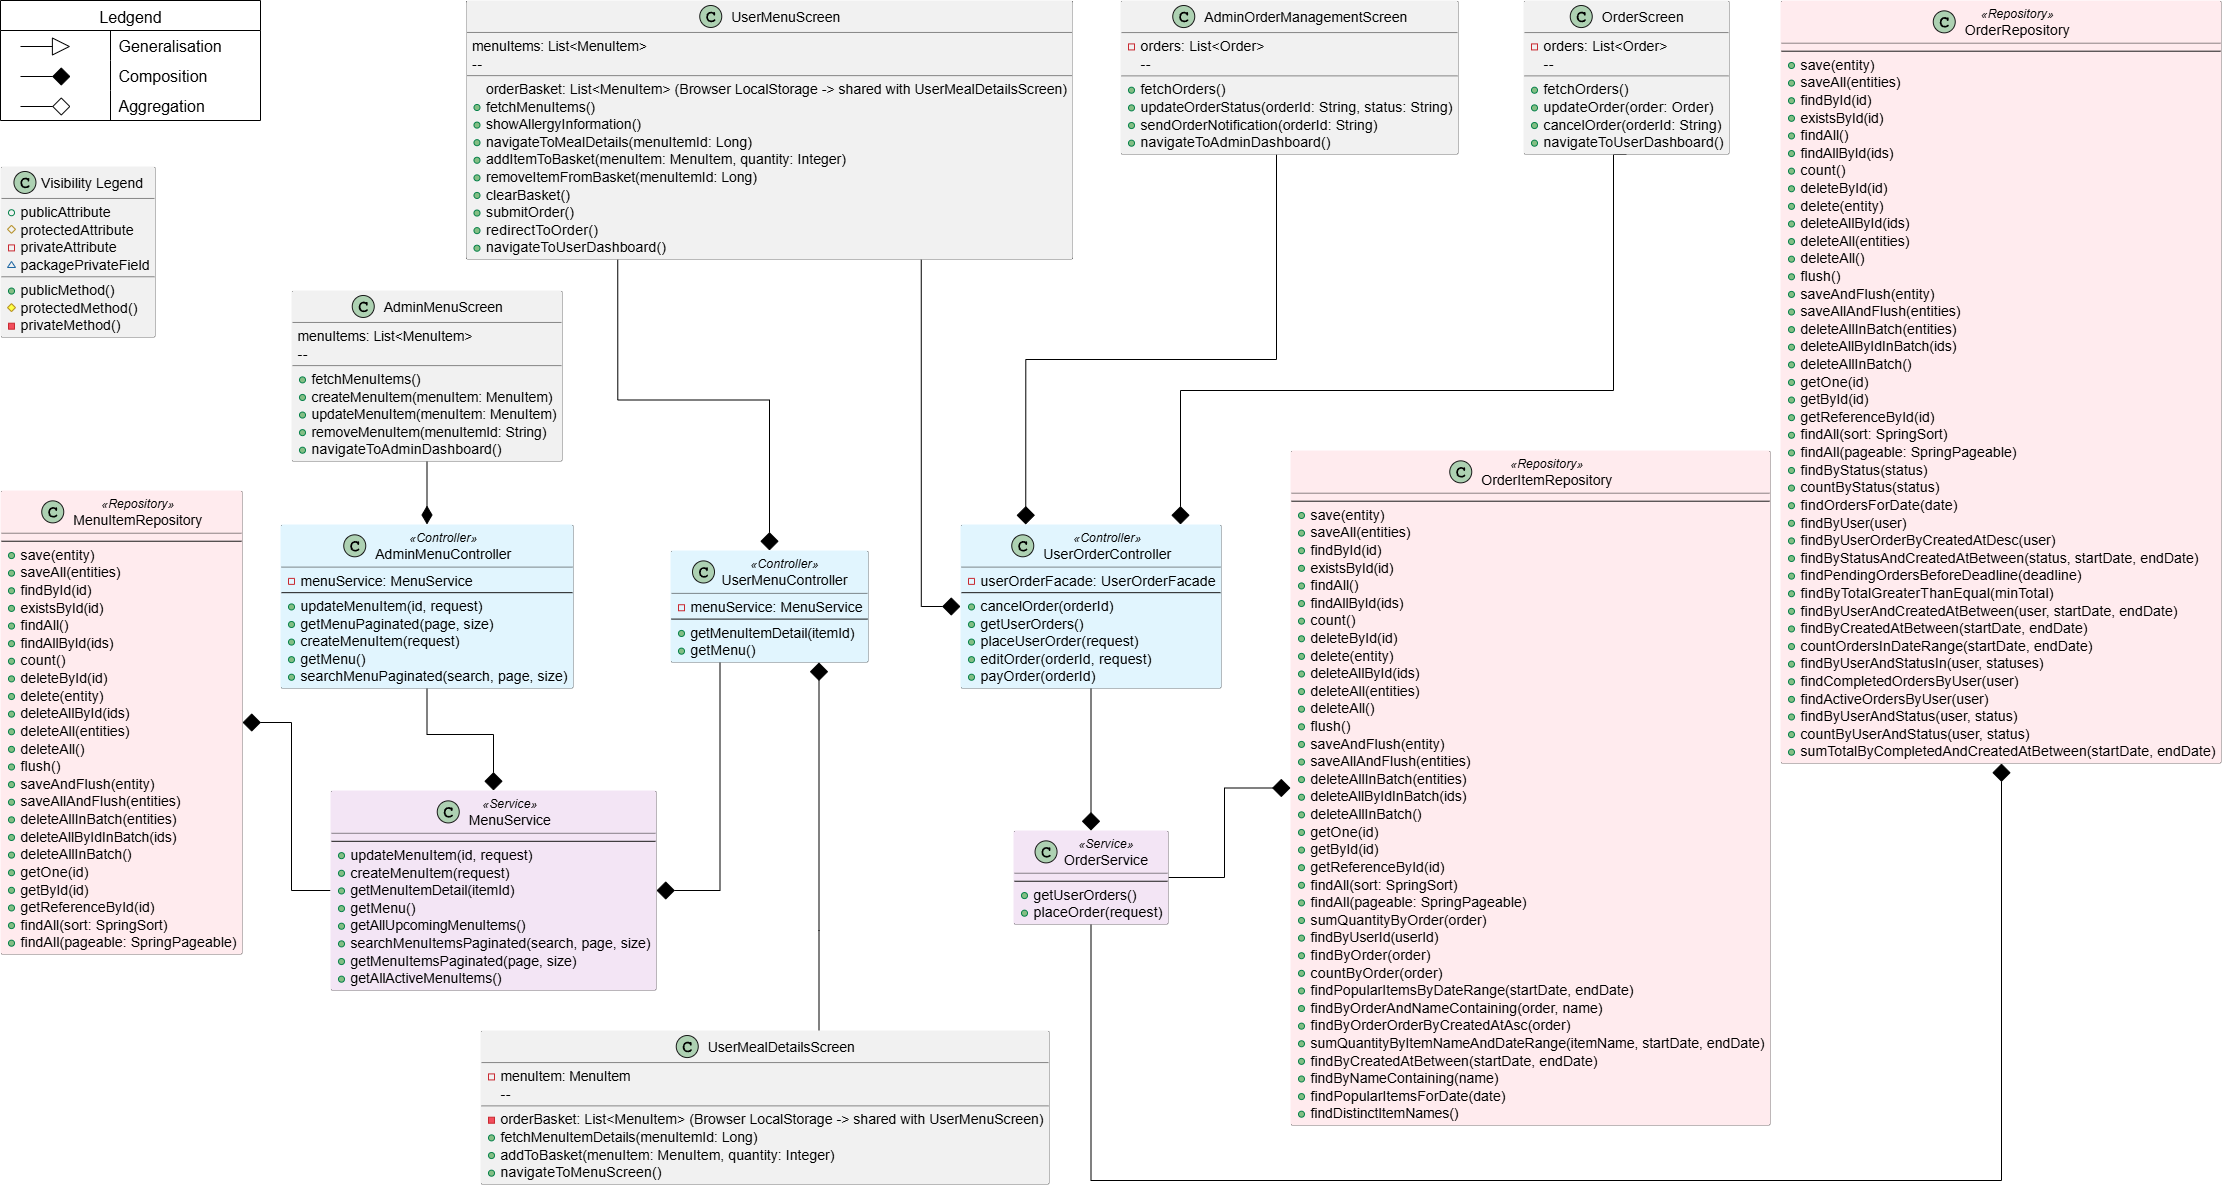
\includegraphics[width=\textwidth]{figures/class_diagrams/menu-order-subsystem.png}
    \caption{Spyskaart en bestelling onderdeel klasdiagram}
    \label{fig:menu_order_subsystem_class_diagram}
\end{figure}

Hier volg die CRC kaarte vir die belangrikste klasse in hierdie
onderdeel.

\textbf{UserMenuScreen} bied gebruikers toegang tot beskikbare spyskaarte, allergie-inligting en die byvoeg van items by die mandjie.
\begin{table}[H]
\centering
\begin{tabular}{|p{0.4\textwidth}|p{0.4\textwidth}|}
    \hline
    \multicolumn{2}{|c|}{\textbf{UserMenuScreen}} \\
    \hline
    \textbf{Verantwoordelikhede} & \textbf{Medewerkers} \\
    \hline
    Wys beskikbare spyskaarte \newline
    Wys allergie-inligting \newline
    Voeg items by bestellingsmandjie \newline
    Navigeer na maaltyd besonderhede
    &
    UserMenuController \\
    \hline
\end{tabular}
\caption{CRC vir UserMenuScreen}
\label{tab:crc_user_menu_screen}
\end{table}

\vspace{1em}
\textbf{AdminOrderManagementScreen} laat administrateurs toe om alle bestellings te besigtig, statusse by te werk en kennisgewings te stuur.
\begin{table}[H]\centering\begin{tabular}{|p{0.4\textwidth}|p{0.4\textwidth}|}
    \hline
    \multicolumn{2}{|c|}{\textbf{AdminOrderManagementScreen}} \\
    \hline
    \textbf{Verantwoordelikhede} & \textbf{Medewerkers} \\
    \hline
    Wys en bestuur alle bestellings \newline
    Werk bestelling status by \newline
    Stuur bestelling kennisgewings \newline
    Filter bestellings volgens kriteria
    &
    UserOrderController \\
    \hline
\end{tabular}
\caption{CRC vir AdminOrderManagementScreen}
\label{tab:crc_admin_order_management_screen}
\end{table}

\vspace{1em}
\textbf{OrderScreen} wys gebruikers se huidige en vorige bestellings, en laat wysigings en kansellasies toe.
\begin{table}[H]\centering\begin{tabular}{|p{0.4\textwidth}|p{0.4\textwidth}|}
    \hline
    \multicolumn{2}{|c|}{\textbf{OrderScreen}} \\
    \hline
    \textbf{Verantwoordelikhede} & \textbf{Medewerkers} \\
    \hline
    Wys gebruiker se huidige en verlede bestellings \newline
    Laat bestelling wysigings en kansellasies toe \newline
    Wys bestelling status en besonderhede
    &
    UserOrderController \\
    \hline
\end{tabular}
\caption{CRC vir OrderScreen}
\label{tab:crc_order_screen}
\end{table}

\vspace{1em}
\textbf{UserOrderController} hanteer alle versoeke rakende gebruikers se bestellings, insluitend plasing, wysiging en betaling.
\begin{table}[H]\centering\begin{tabular}{|p{0.4\textwidth}|p{0.4\textwidth}|}
    \hline
    \multicolumn{2}{|c|}{\textbf{UserOrderController}} \\
    \hline
    \textbf{Verantwoordelikhede} & \textbf{Medewerkers} \\
    \hline
    Hanteer gebruiker bestelling versoeke \newline
    Verwerk bestelling plasings \newline
    Hanteer bestelling wysigings en kansellasies \newline
    Verwerk bestelling betalings
    &
    OrderService \\
    \hline
\end{tabular}
\caption{CRC vir UserOrderController}
\label{tab:crc_user_order_controller}
\end{table}

\vspace{1em}
\textbf{OrderService} verwerk besigheidslogika vir bestellings, valideer inligting, bereken totale en bestuur statusse.
\begin{table}[H]\centering\begin{tabular}{|p{0.4\textwidth}|p{0.4\textwidth}|}
    \hline
    \multicolumn{2}{|c|}{\textbf{OrderService}} \\
    \hline
    \textbf{Verantwoordelikhede} & \textbf{Medewerkers} \\
    \hline
    Verwerk bestelling besigheidslogika \newline
    Valideer bestelling inligting \newline
    Bereken bestelling totale \newline
    Bestuur bestelling status veranderinge
    &
    OrderItemRepository \newline
    OrderRepository \\
    \hline
\end{tabular}\end{table}

\vspace{1em}
\textbf{UserMealDetailsScreen} wys gedetailleerde maaltydinligting, voedingswaarde, beelde en voeg maaltye by die mandjie.
\begin{table}[H]\centering\begin{tabular}{|p{0.4\textwidth}|p{0.4\textwidth}|}
    \hline
    \multicolumn{2}{|c|}{\textbf{UserMealDetailsScreen}} \\
    \hline
    \textbf{Verantwoordelikhede} & \textbf{Medewerkers} \\
    \hline
    Wys gedetailleerde maaltyd inligting \newline
    Wys voedingswaarde en allergie-inligting \newline
    Wys maaltyd beelde \newline
    Voeg maaltyd by bestellingsmandjie
    &
    UserMenuController \\
    \hline
\end{tabular}
\caption{CRC vir UserMealDetailsScreen}
\label{tab:crc_user_meal_details_screen}
\end{table}

\vspace{1em}
\textbf{UserMenuController} hanteer gebruikers se spyskaartversoeke, verskaf maaltydbesonderhede en bestuur filters.
\begin{table}[H]\centering\begin{tabular}{|p{0.4\textwidth}|p{0.4\textwidth}|}
    \hline
    \multicolumn{2}{|c|}{\textbf{UserMenuController}} \\
    \hline
    \textbf{Verantwoordelikhede} & \textbf{Medewerkers} \\
    \hline
    Hanteer spyskaart versoeke vir gebruikers \newline
    Verskaf maaltyd besonderhede \newline
    Hanteer spyskaart filters en soeke
    &
    MenuService \\
    \hline
\end{tabular}\end{table}

\vspace{1em}
\textbf{AdminMenuController} hanteer administratiewe spyskaartversoeke, skep en wysig items, en bestuur gepagineerde vertoning.
\begin{table}[H]\centering\begin{tabular}{|p{0.4\textwidth}|p{0.4\textwidth}|}
    \hline
    \multicolumn{2}{|c|}{\textbf{AdminMenuController}} \\
    \hline
    \textbf{Verantwoordelikhede} & \textbf{Medewerkers} \\
    \hline
    Hanteer administratiewe spyskaart versoeke \newline
    Skep en wysig spyskaart items \newline
    Verwyder spyskaart items \newline
    Bestuur spyskaart gepagineerde vertoning
    &
    MenuService \\
    \hline
\end{tabular}
\caption{CRC vir AdminMenuController}
\label{tab:crc_admin_menu_controller}
\end{table}

\vspace{1em}
\textbf{AdminMenuScreen} bied administrateurs die vermoë om spyskaartitems te bestuur, te skep, te wysig en te verwyder.
\begin{table}[H]\centering\begin{tabular}{|p{0.4\textwidth}|p{0.4\textwidth}|}
    \hline
    \multicolumn{2}{|c|}{\textbf{AdminMenuScreen}} \\
    \hline
    \textbf{Verantwoordelikhede} & \textbf{Medewerkers} \\
    \hline
    Wys en bestuur spyskaart items \newline
    Skep nuwe spyskaart items \newline
    Wysig bestaande spyskaart items \newline
    Verwyder spyskaart items
    &
    AdminMenuController \\
    \hline
\end{tabular}
\caption{CRC vir AdminMenuScreen}
\label{tab:crc_admin_menu_screen}
\end{table}

\vspace{1em}
\textbf{MenuService} bestuur die besigheidslogika van die spyskaart, verkry items met filters, valideer en hanteer CRUD-operasies.
\begin{table}[H]\centering\begin{tabular}{|p{0.4\textwidth}|p{0.4\textwidth}|}
    \hline
    \multicolumn{2}{|c|}{\textbf{MenuService}} \\
    \hline
    \textbf{Verantwoordelikhede} & \textbf{Medewerkers} \\
    \hline
    Bestuur spyskaart besigheidslogika \newline
    Verkry spyskaart items met filters \newline
    Valideer spyskaart item inligting \newline
    Hanteer spyskaart item CRUD operasies
    &
    MenuItemRepository \\
    \hline
\end{tabular}
\caption{CRC vir MenuService}
\label{tab:crc_menu_service}
\end{table}

